\setlength{\columnsep}{3pt}
\begin{flushleft}
	\bigskip
	\begin{itemize}
		\item The cron daemon runs jobs/processes on your system at a scheduled date/time.
		\item Cron daemon reads the \textbf{crontab (cron tables)} for commands and scripts.
		\item Every user can set crontab for themself.
		\item Crontab related files:
 
		\begin{itemize}
			\item Configuration file for crontab: \textbf{/etc/crontab}
			\item User specific crontab files: \textbf{/var/spool/cron/\{user\_name\}}
			\item Cron log file: \textbf{/var/log/cron}
		\end{itemize}
		
		\item Syntax of crontab jobs:
		
		\begin{figure}[h!]
			\centering
			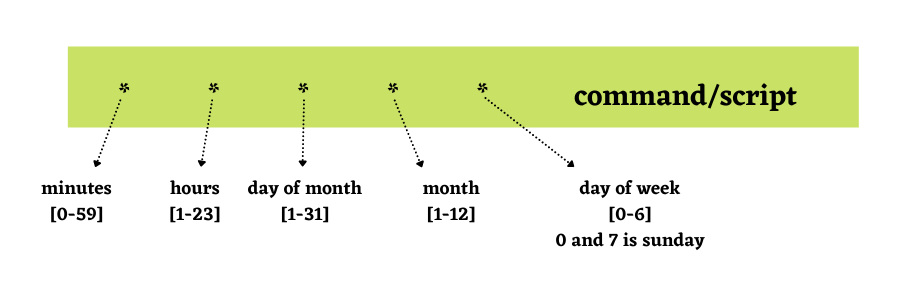
\includegraphics[scale=0.5]{content/chapter13/images/cronjob.png}
			
			\caption{crontab file syntax}
			\label{fig:cronjob}
		\end{figure}
	\end{itemize}
	
	
\end{flushleft}

\newpage





